\documentclass[tikz,border=6pt]{standalone}
\usepackage{amsmath,amssymb}
\usepackage{xcolor}
\definecolor{accent}{HTML}{1F4E79}
\definecolor{accent2}{HTML}{2B5F6B}
\definecolor{muted}{HTML}{5A564F}
\definecolor{panel}{HTML}{F8F6F0}
\definecolor{linecol}{HTML}{D8D2C4}
\definecolor{ink}{HTML}{1E1C1A}
\definecolor{astroblue}{HTML}{1B4F72}
\definecolor{sunyellow}{HTML}{E8A33D}
\definecolor{bodyA}{HTML}{A13D2C}
\usetikzlibrary{calc,arrows.meta}
\usepackage[T1]{fontenc}\usepackage{newpxtext,newpxmath}
% #1 relative semi-major axis (cm)  #2 e  #3 share of body 1 (m2/M)  #4 share of body 2 (m1/M)
% path of body k is (share) a(1-e^2)/(1+e cos v) (cos v, sin v), body 2 with a minus sign
\newcommand{\paths}[4]{%
  \draw[\ca,line width=0.7pt,samples=120,domain=0:360,smooth,variable=\v]
    plot ({#3*#1*(1-#2*#2)/(1+#2*cos(\v))*cos(\v)},{#3*#1*(1-#2*#2)/(1+#2*cos(\v))*sin(\v)});
  \draw[\cb,line width=0.7pt,samples=120,domain=0:360,smooth,variable=\v]
    plot ({-#4*#1*(1-#2*#2)/(1+#2*cos(\v))*cos(\v)},{-#4*#1*(1-#2*#2)/(1+#2*cos(\v))*sin(\v)});
  % same sense of motion on both paths (increasing v)
  \draw[\ca,-{Stealth[length=5pt]},line width=0.7pt,samples=3,domain=262:266,variable=\v]
    plot ({#3*#1*(1-#2*#2)/(1+#2*cos(\v))*cos(\v)},{#3*#1*(1-#2*#2)/(1+#2*cos(\v))*sin(\v)});
  \draw[\cb,-{Stealth[length=5pt]},line width=0.7pt,samples=3,domain=262:266,variable=\v]
    plot ({-#4*#1*(1-#2*#2)/(1+#2*cos(\v))*cos(\v)},{-#4*#1*(1-#2*#2)/(1+#2*cos(\v))*sin(\v)});
}
% numbered moment at true anomaly #5: #1 a, #2 e, #3 share1, #4 share2, #5 v, #6 number
\newcommand{\moment}[6]{%
  \pgfmathsetmacro{\rr}{#1*(1-#2*#2)/(1+#2*cos(#5))}
  \draw[muted,dashed,line width=0.3pt] ({-#4*\rr*cos(#5)},{-#4*\rr*sin(#5)}) -- ({#3*\rr*cos(#5)},{#3*\rr*sin(#5)});
  \node[circle,fill=\ca,text=white,inner sep=0.6pt,minimum size=9pt,font=\fontsize{6}{6}\selectfont] at ({#3*\rr*cos(#5)},{#3*\rr*sin(#5)}) {#6};
  \node[circle,fill=\cb,text=white,inner sep=0.6pt,minimum size=9pt,font=\fontsize{6}{6}\selectfont] at ({-#4*\rr*cos(#5)},{-#4*\rr*sin(#5)}) {#6};
}
\def\ca{bodyA}\def\cb{astroblue}
\newcommand{\cm}{\draw[ink,line width=0.6pt] (-0.1,-0.1)--(0.1,0.1) (-0.1,0.1)--(0.1,-0.1);}
\begin{document}
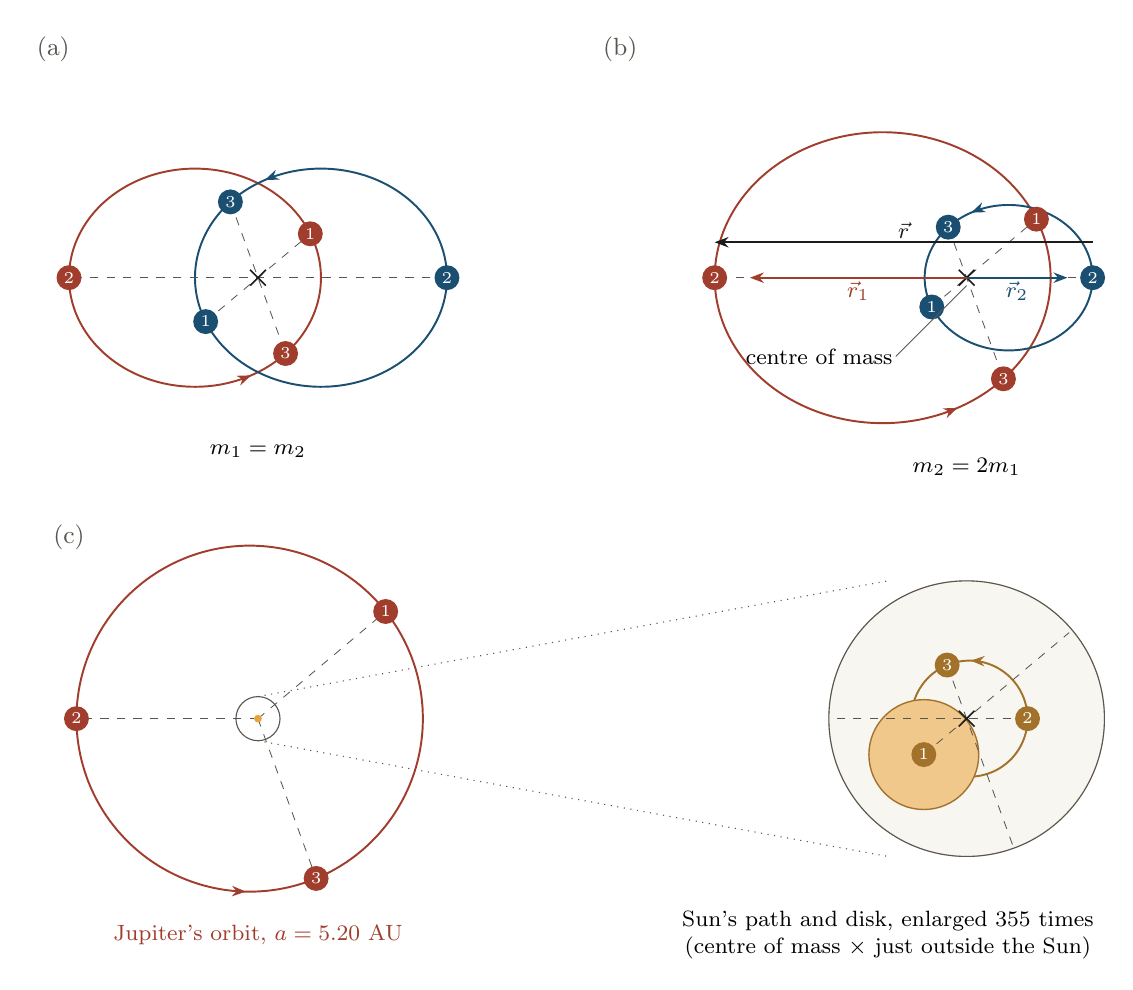
\begin{tikzpicture}[font=\small]
\tikzset{lab/.style={font=\footnotesize,inner sep=1pt}}
% ---------- (a) equal masses
\begin{scope}
  \paths{3.2}{0.5}{0.5}{0.5}
  \moment{3.2}{0.5}{0.5}{0.5}{40}{1}
  \moment{3.2}{0.5}{0.5}{0.5}{180}{2}
  \moment{3.2}{0.5}{0.5}{0.5}{290}{3}
  \cm
  \node[muted] at (-2.6,2.9) {(a)};
  \node[lab] at (0,-2.2) {$m_1=m_2$};
\end{scope}
% ---------- (b) m2 = 2 m1
\begin{scope}[xshift=9cm]
  \paths{3.2}{0.5}{0.6666667}{0.3333333}
  \moment{3.2}{0.5}{0.6666667}{0.3333333}{40}{1}
  \moment{3.2}{0.5}{0.6666667}{0.3333333}{180}{2}
  \moment{3.2}{0.5}{0.6666667}{0.3333333}{290}{3}
  \cm
  % vectors at moment 2
  \pgfmathsetmacro{\rr}{3.2*0.75/(1+0.5*cos(180))}
  \pgfmathsetmacro{\xa}{0.6666667*\rr*cos(180)} \pgfmathsetmacro{\ya}{0.6666667*\rr*sin(180)}
  \pgfmathsetmacro{\xb}{-0.3333333*\rr*cos(180)} \pgfmathsetmacro{\yb}{-0.3333333*\rr*sin(180)}
  \pgfmathsetmacro{\nx}{sin(180)*0.45} \pgfmathsetmacro{\ny}{-cos(180)*0.45}
  \draw[-{Stealth[length=5pt]},ink,line width=0.8pt] ({\xb+\nx},{\yb+\ny}) -- node[lab,above,pos=0.5] {$\vec r$} ({\xa+\nx},{\ya+\ny});
  \draw[-{Stealth[length=5pt]},bodyA,line width=0.8pt] (0,0) -- ({0.86*\xa},{0.86*\ya}) node[lab,below,pos=0.5,bodyA] {$\vec r_1$};
  \draw[-{Stealth[length=5pt]},astroblue,line width=0.8pt] (0,0) -- ({0.8*\xb},{0.8*\yb}) node[lab,below,pos=0.5,astroblue] {$\vec r_2$};
  \draw[muted,line width=0.3pt] (0,-0.1) -- (-0.9,-1.0); \node[lab,anchor=east] at (-0.9,-1.0) {centre of mass};
  \node[muted] at (-4.4,2.9) {(b)};
  \node[lab] at (0,-2.4) {$m_2=2m_1$};
\end{scope}
% ---------- (c) Sun and Jupiter
\begin{scope}[yshift=-5.6cm]
  \node[muted] at (-2.4,2.3) {(c)};
  % Jupiter orbit at small scale (a = 5.20 AU drawn 2.2 cm)
  \def\ca{bodyA}
  \draw[bodyA,line width=0.7pt,samples=100,domain=0:360,smooth,variable=\v]
    plot ({2.2*(1-0.048*0.048)/(1+0.048*cos(\v))*cos(\v)},{2.2*(1-0.048*0.048)/(1+0.048*cos(\v))*sin(\v)});
  \foreach \v/\n in {40/1,180/2,290/3}{
    \pgfmathsetmacro{\rr}{2.2*(1-0.048*0.048)/(1+0.048*cos(\v))}
    \draw[muted,dashed,line width=0.3pt] (0,0) -- ({\rr*cos(\v)},{\rr*sin(\v)});
    \node[circle,fill=bodyA,text=white,inner sep=0.6pt,minimum size=9pt,font=\fontsize{6}{6}\selectfont] at ({\rr*cos(\v)},{\rr*sin(\v)}) {\n};}
  \draw[bodyA,-{Stealth[length=5pt]},line width=0.7pt,samples=3,domain=262:266,variable=\v]
    plot ({2.2*(1-0.048*0.048)/(1+0.048*cos(\v))*cos(\v)},{2.2*(1-0.048*0.048)/(1+0.048*cos(\v))*sin(\v)});
  \fill[sunyellow] (0,0) circle (1.4pt);
  \node[lab,bodyA] at (0,-2.75) {Jupiter's orbit, $a=5.20$ AU};
  \draw[muted,line width=0.4pt] (0,0) circle (0.28);
  % zoomed inset, 150 cm per AU, so Jupiter's orbit is drawn 355 times larger than in the main panel (150 vs 0.423 cm per AU)
  \begin{scope}[xshift=9cm]
    \draw[linecol,line width=0.4pt,fill=panel] (0,0) circle (1.75);
    \draw[muted,line width=0.4pt] (0,0) circle (1.75);
    \begin{scope}
      \clip (0,0) circle (1.75);
      \pgfmathsetmacro{\sh}{1/1049}
      % Sun's centre path (share m_J/M of Jupiter's orbit, drawn at 150 cm/AU)
      \draw[sunyellow!70!black,line width=0.7pt,samples=120,domain=0:360,smooth,variable=\v]
        plot ({-\sh*780*(1-0.048*0.048)/(1+0.048*cos(\v))*cos(\v)},{-\sh*780*(1-0.048*0.048)/(1+0.048*cos(\v))*sin(\v)});
      % Sun's disk at moment 1
      \pgfmathsetmacro{\rr}{\sh*780*(1-0.048*0.048)/(1+0.048*cos(40))}
      \fill[sunyellow!60] ({-\rr*cos(40)},{-\rr*sin(40)}) circle (0.6975);
      \draw[sunyellow!70!black,line width=0.5pt] ({-\rr*cos(40)},{-\rr*sin(40)}) circle (0.6975);
      \foreach \v/\n in {40/1,180/2,290/3}{
        \pgfmathsetmacro{\rr}{\sh*780*(1-0.048*0.048)/(1+0.048*cos(\v))}
        \draw[muted,dashed,line width=0.3pt] ({-\rr*cos(\v)},{-\rr*sin(\v)}) -- ({1.7*cos(\v)},{1.7*sin(\v)});
        \node[circle,fill=sunyellow!70!black,text=white,inner sep=0.6pt,minimum size=9pt,font=\fontsize{6}{6}\selectfont] at ({-\rr*cos(\v)},{-\rr*sin(\v)}) {\n};}
      \draw[sunyellow!70!black,-{Stealth[length=5pt]},line width=0.7pt,samples=3,domain=262:266,variable=\v]
        plot ({-\sh*780*(1-0.048*0.048)/(1+0.048*cos(\v))*cos(\v)},{-\sh*780*(1-0.048*0.048)/(1+0.048*cos(\v))*sin(\v)});
    \end{scope}
    \cm
  \end{scope}
  \draw[muted,dotted,line width=0.4pt] (0,0.28) -- (8,1.75);
  \draw[muted,dotted,line width=0.4pt] (0,-0.28) -- (8,-1.75);
  \node[lab,align=center] at (8,-2.75) {Sun's path and disk, enlarged 355 times\\(centre of mass $\times$ just outside the Sun)};
\end{scope}
\end{tikzpicture}
\end{document}
